\documentclass{article}
\usepackage{graphicx} % Required for inserting images
\title{D4: Sviluppo Applicazione}
\author{G06}
\usepackage{fancyhdr}
\usepackage{hyperref}
\usepackage{array}
\usepackage{float}
\newcommand{\myheaderimage}{\includegraphics[width=2cm]{D3/Images/LogoEasyLib.png}}
\pagestyle{fancy}
\fancyhf{} % Clear the header and footer
\lhead{\myheaderimage} % Place the image in the top right corner
\setlength{\headheight}{3cm} % Adjust the height as needed
\rhead{D4-G06}

\begin{document}


\maketitle
\tableofcontents
\newpage



\section{Scopo del documento}

In questo documento vengono descritte tutte le informazioni di sviluppo dell'applicazione \textbf{EasyLib}.\\
Nello specifico vengono trattate tutte le parti di login, gestione, e noleggi alla nostra biblioteca digitale, iniziando dalle descrizione degli User Flows, sia per l'utente normale che per l'amministratore; per poi passare alla struttura del codice scritto, con la descrizione di tutte le varie API sviluppate. Ogni API creata verrà analizzata nelle sue funzioni, avendo la sua documentazione, e poi, nella sezione testing avrà i risultati dei test a cui è stata sottoposta.
Per concludere è presente una sezione che descrive il deployment dell'applicazione e tutte le informazione del Git Repository.

\section{User Flows}

Lo User flow rappresenta come l'utente interagisce con il design del frontend, e le azioni che può compiere spostandosi tra le varie pagine dell'applicazione.
Per prima cosa introduciamo la legenda del diagramma che ci permette di rappresentare lo user flow.
\begin{figure}[H]
     \centering
     \includegraphics[width=130mm]{D4/Images/Legenda.png}
     \caption{Legenda User Flow}
    \end{figure}
\footnote{Per visualizzare le foto con una qualità maggiore si visiti il seguente link \url{https://drive.google.com/drive/folders/1mCccEUUQHTccKQIxqfn6cw_KfOJ2SWsW?usp=sharing}}

Informazioni sulla legenda:
\begin{itemize}
    \item con \textbf{Bivio} si intende un  punto in cui la risposta del sistema può variare a seconda della selezione dell'utente.
    \item per \textbf{Attesa} si intende un  punto in cui il sistema rimette all'utente la decisione su cosa fare: se ripetere un operazione appena compiuto o tornare indietro alla pagina precedente e effettuare altre azioni.
    \item per \textbf{Arrivo} si intende il momento in cui il sistema ha soddisfatto le richieste dell'utente. Nel nostro caso per l'utente il punto di 'Arrivo' corrisponde con la ricerca ed eventuale noleggio di un libro, mentre per l'admin corrisponde con la creazione di una multa, l'aggiunta di un nuovo libro al database o la conferma del reso di un libro da parte di un utente.
\end{itemize}

Per rendere più chiaro l'intero diagramma e non saturarlo di collegamenti, abbiamo optato per creare 2 User flow diversi: il primo riguardante le funzionalità dell'\textbf{utente normale}; mentre il secondo rappresenta le azioni che possono essere svolte da un \textbf{utente Admin} in possesso delle dovute credenziali.

\subsection{User Flow Utente}

\begin{figure}[H]
    \centering
    \includegraphics[width=130mm]{D4/Images/userFlowUtente.png}
    \caption{User Flow utente}
\end{figure}

\subsection{User Flow Admin}

\begin{figure}[H]
    \centering
    \includegraphics[width=130mm]{{D4/Images/userFlowAdmin.png}}
    \caption{User flow Admin}
\end{figure}

\section{Application implementation and documentation}
Nei documenti precedenti vengono descritti tutte le funzionalità e i requisiti che la nostra applicazione EasyLib deve avere.
In questa sezione invece verrà descritto come queste funzionalità sono state sviluppate tramite. 
Lo sviluppo dell'applicazione  è stato creato usando HTML, CSS, Javascript e NodeJs; mentre la gestione dei database necessari all'uso dell'applicazione è stato usato MongoDB.

\subsection{Struttura}
La struttura del progetto è rappresentata nella seguente immagine
\begin{figure}[H]
    \centering
    \includegraphics[width=80mm]{D4/Images/StrutturaProject.png}
    \caption{Struttura del progetto}
\end{figure}

Nella cartella \textbf{auxiliares} sono presenti delle funzioni per verificare che la password rispetti i requisiti (lunghezza maggiore o uguale  a 8 caratteri, e almeno un carattere speciale) e che la stringa inserita nei campi mail sia effettivamente una mail valida.
La cartella \textbf{controllers} contiene le varie api sviluppate divise per i modelli utilizzati. Tutta la parte riguardante il FrontEnd, è contenuta nella cartella \textbf{Frontend} dove sono collocati tutti i file CSS e HTML. 
I modelli con i loro attributi descritti in seguito in questo documento sono contenuti nella cartella \textbf{models};
la cartella \textbf{Test} contiene i vari test svolti sulle varie API, e sono implementati tramite Jest. La cartella \textbf{routes} infine definisce il percorso e la tipologia delle varie API create.
Oltre alle cartelle ci sono alcuni file :
\begin{itemize}
    \item \textbf{Swagger.json} dove sono descritte con tanto di esempi le API sviluppate per il progetto.
    \item \textbf{index.js} è il programma che deve essere eseguito per instaurare la connessione con MongoDB e attivare il server all'indirizzo localhost.
    \item \textbf{Package.json} contiene il file di configurazione generale del progetto.
    \item \textbf{.env} E' il file in cui sono definite le variabili dell'ambiente.
    \item \textbf{server.js} che importa tutti i moduli utilizzati nel Back-end e definisce gli end-point delle API.
\end{itemize}.

\subsection{Dependencies del progetto}
Qui sono descritti i moduli Node aggiunti a package.json nell'area dependencies, tra cui:
\begin{itemize}
    \item cors: modulo per permettere alla web app di supportare il Cross-Origin Resource Sharing protocol
    \item dotenv: permette di utilizzare le variabile d’ambiente definite nel file .env
    \item express: framework che offre molte funzioni per la gestione di API per le web application.
    \item jsonwebtoken: modulo per creare e gestire un token d’accesso.
    \item mongoose: fornisce le varie funzioni per interagire con MongoDB.
    \item multer: gestisce il body nelle varie API.
    \item swagger-ui-express: tool usato per documentare e testare la API che abbiamo progettato.
    \item jest: modulo usato per il testing delle API e delle funzioni nel back-end.
    \item supertest: modulo usato per chiamare le API in fase di testing.
\end{itemize}


\subsection{Modelli nel database}
Per la gestione dei dati abbiamo creato 5 collezioni principali:
\begin{enumerate}
    \item \textbf{Utente:} che contiene tutte le informazioni relative ai vari utenti registrati.
    I campi ID, Nome, cognome, mail e password che vengono inseriti alla prima registrazione.\\ 
    \textit{Libri\_noleggiati} Dove sono presenti gli ID univoci dei vari libri noleggiati da un singolo utente.\\
    E \textit{n\_libri} che serve per rispettare il RF8 che permette il noleggio di al più 5 libri.\\
    
    Viene mostrato prima lo schema del modello creato per utente: 
        \begin{figure}[H]
        \centering
        \includegraphics[width=80mm]{D4/Images/ModelUtente.png}
        \caption{Modello utente}
    \end{figure}
    
    E successivamente  vengono riportati degli esempi delle collezioni utente nel database, di un utente  registrato e uno in possesso di credenziali admin per poter provare entrambe le interfacce.
    \begin{figure}[H]
        \centering
        \includegraphics[width=130mm]{D4/Images/utenteDB.png}
        \caption{Tipo di dato: Utente}
    \end{figure}
    \begin{figure}[H]
        \centering
        \includegraphics[width=130mm]{D4/Images/UtenteAdminDB.png}
        \caption{Tipo di dato: Utente Admin}
    \end{figure}
    \item \textbf{Appuntamenti:} in cui sono salvate le informazioni degli appuntamenti effettuati dagli utenti.
    Gli attributi necessari sono la mail dell'utente che deve essere registrato, la \textit{Data} richiesta per l'appuntamento e il \textit{tipo\_app} che descrive la tipologia dell'appuntamento desiderata e può essere un ritiro, un reso o una donazione.
     Sotto viene mostrato il modello creato.
    \begin{figure}[H]
        \centering
        \includegraphics[width=80mm]{D4/Images/ModelAppuntamento.png}
        \caption{Modello Appuntamento}
    \end{figure}

    E successivamente un esempio del tipo di dato Appuntamento presente all'interno del database:
    \begin{figure}[H]
        \centering
        \includegraphics[width=130mm]{D4/Images/AppDB.png}
        \caption{Tipo di dato: Appuntamento}
    \end{figure}
    
    \item \textbf{Libri:} dove vengono salvati tutti i vari volumi presenti su \textbf{EasyLib}.
    Gli attributi del modello sono le caratteristiche di ogni volume, tra cui il titolo, il nome e cognome dell'autore e il genere, necessari per la ricerca nell'archivio e filtri di ricerca. Un ID del libro creato automaticamente e sequenziale aggiunto dal sistema all'inserimento di ogni nuovo libro.
    Inoltre è presente una \textit{Scadenza}  del noleggio, che è settata a NULL se il libro non è in noleggio; infine \textit{Is\_available} serve per gestire la disponibilità del libro in caso di ritiro.
    
    Qui sotto viene riportato il modello Book creato:
    \begin{figure}[H]
        \centering
        \includegraphics[width=80mm]{D4/Images/ModelBook.png}
        \caption{Modello Book}
    \end{figure}

    E di seguito è rappresentata un immagine di esempio del tipo di dato Book all'interno del database:
    
    \begin{figure}[H]
        \centering
        \includegraphics[width=130mm]{D4/Images/LibroDB.png}
        \caption{Tipo di dato: Libro}
    \end{figure}

    \item \textbf{Multa:} in cui vengono riportate le informazioni riguardanti le varie contravvenzioni.
    Gli attributi del modello sono: la mail a cui è legata la multa, l'\textit{importo} della multa e la data entro cui bisogna pagare la multa,  contenuta in \textit{paga entro}.
    
    Prima è raffigurata un immagine del modello Multa creato:
        \begin{figure}[H]
        \centering
        \includegraphics[width=80mm]{D4/Images/ModelMulta.png}
        \caption{Modello Multa}
    \end{figure}

    E poi un esempio del tipo di dato multa all'interno del database:
    
    \begin{figure}[H]
        \centering
        \includegraphics[width=130mm]{D4/Images/multaDB.png}
        \caption{Tipo di dato: Multa}
    \end{figure}
\end{enumerate}

\subsection{API del progetto}
In questa sottosezione del documento vengono descritte le varie API implementate a partire dal diagramma delle classi mostrato nel documento D3-G06. Useremo un diagramma per rappresentare l’estrazione delle risorse a partire dal class diagram e uno per rappresentare le risorse sviluppate.

\subsubsection{Estrazione delle risorse}
Questi diagrammi presentano come abbiamo estratto le risorse partendo dal class diagram.\\
Abbiamo diviso le risorse per la parte utente e quella dell'admin, individuando dal diagramma delle classi dei modelli, i cui attributi sono necessari per la memorizzazione nel database.\\
Abbiamo convertito i metodi delle classi estratte in API, che pensavamo definissero meglio lo scheletro del progetto.
Di queste, nei diagrammi sottostanti viene definito il tipo di API (GET, POST, PATCH, DELETE)e con quali attributi interagiscono.\\
Inoltre abbiamo etichettato ogni API in base alla loro interazione con Frontend e Backend; nel caso delle API di tipo GET l'effetto più immediato sarà quello sul Frontend, le restanti  POST, PATCH e DELETE invece, avranno un interazione più profonda sul Backend in quanto andaranno a modificare, creare e cancellare risorse nel database.

\begin{figure}[H]
    \centering
    \includegraphics[width=130mm]{D4/Images/UtenteAPIExtraction.jpeg}
    \caption{Estrazione risorse relative all'utente}
\end{figure}

\begin{figure}[H]
    \centering
    \includegraphics[width=130mm]{D4/Images/AdminAPIExtraction.jpeg}
    \caption{Estrazione risorse relative all'Admin}
\end{figure}

\subsubsection{Diagramma delle risorse}
Nel seguenti diagramma abbiamo rappresentato in maniera più specifica le API sviluppate nel progetto.
il diagramma è stato diviso, per permettere più chiarezza e non creare un immagine troppo compatta, in una parte, come nell'estrazione delle risorse appena descritto, in sezione admin e sezione utente; la seconda parte invece descrive le API a partire dal  modello appuntamento e dal modello book.\\ Si è specificato per ogni interfaccia un input e un output possibile, in base alla correttezza o meno dell'esecuzione dell'API.

\begin{figure}[H]
    \centering
    \includegraphics[width=130mm]{D4/Images/UtenteResourceModel.jpeg}
    \caption{Diagramma delle risorse: Sezione utente}

\end{figure}

\begin{figure}[H]
    \centering
    \includegraphics[width=130mm]{D4/Images/AdminResourceModel.jpeg}
    \caption{Diagramma delle risorse: Sezione Admin}

\end{figure}

\begin{figure}[H]
    \centering
    \includegraphics[width=130mm]{D4/Images/BookResourceModel.jpeg}
    \caption{Diagramma delle risorse: parte Book}

\end{figure}

\begin{figure}[H]
    \centering
    \includegraphics[width=130mm]{D4/Images/AppuntementoResourceModel.jpeg}
    \caption{Diagramma delle risorse: parte appuntamento}
\end{figure}


\subsection{Sviluppo delle API}
In questa parte verranno descritti i funzionamenti di tutte le API implementate del progetto. 
Viene riportato con delle immagini solo un esempio di API per ogni tipologia (GET, POST, PATCH e DELETE) perché il codice è molto lungo e saturerebbe il documento di immagini.in ogni caso il codice corrispondente a tutte le altre interfacce può essere trovato nella repository del Backend, nella cartella \textbf{controllers}, divise in più file.

\subsubsection{API del modello utente}
Sotto descritte le API relative alle varie azioni possibili sulla risorsa Utente.

\vspace{0.5cm}

\noindent \textbf{SignUp}\\
L'API SignUp viene utilizzata per creare un nuovo utente, riceve in input un body con i dati del nuovo utente da registrare: nome cognome, mail, password, tutti necessari.
Restituisce in output l'utente creato se non ci sono stati errori, oppure vari messaggi di errore, ad esempio "mail o password non valida" "mail già in uso".
Si utilizza il metodo findOne() per verificare l'unicità della mail, il modello ausiliare Counter per assegnare un ID univoco per ogni utente e il metodo save() per salvare la risorsa nel database.\\

\noindent \textbf{Creazione di un appuntamento}\\
L'API createApp viene utilizzata per creare un nuovo appuntamento, riceve in input un body con i dati necessari per creare l'appuntamento: mail dell'utente, data dell'appuntamento, e il tipo di appuntamento( donazione, ritiro e restituzione) tutti necessari.
Restituisce in output l'appuntamento creato se non ci sono stati errori, oppure vari messaggi di errore.
Si utilizza il metodo findOne() per trovare l'utente che desidera creare un nuovo appuntamento e il metodo save() per salvare la risorsa nel database. Può essere usata da utenti che hanno effettuato il login.\\

\begin{figure}[H]
    \centering
    \includegraphics[width=120mm]{D4/Images/APIPost.png}
    \caption{createApp: API POST}
\end{figure}

\noindent \textbf{Cancellazione di un appuntamento}\\
L'API deleteApp viene utilizzata per cancellare un appuntamento di cui un utente non vuole usufruire.
Riceve in input la mail dell'utente e ritorna in output un messaggio  di cancellazione avvenuta con successo o un errore vario.
Si utilizza il metodo findOne() per trovare l'utente che desidera cancellare un appuntamento. Può essere usata da utenti che hanno effettuato il login.\\

\noindent \textbf{Trova i Libri noleggiati da un utente}\\
L'API getBooks viene utilizzata per vedere i libri noleggiati da un utente, viene preso in input la mail dell'utente e ritorna l'elenco dei libri, sotto forma di array, in possesso di un utente se non ha problemi; mentre ritorna errori vari se l'input non è corretto.
Si utilizza il metodo findOne() per trovare la mail dell'utente di cui ritornare la lista dei libri. I libri vengono cercati dall'API tramite l'id del libro, che poi viene utilizzato per stampare le informazioni dei volumi (titolo, nome e cognome dell'autore, genere e scadenza del noleggio). Può essere usata da utenti che hanno effettuato il login.\\

\begin{figure}[H]
    \centering
    \includegraphics[width=120mm]{D4/Images/APIGet.png}
    \caption{getBooks: API GET}
\end{figure}

\noindent \textbf{Noleggiare un libro}\\
L'API RentedBooks serve per poter noleggiare un libro, e di conseguenza inserire il libro all'interno dei libri noleggiati dall'utente, settare la scadenza del noleggio e modificare la disponibilità del libro a FALSE.
Viene usato il metodo updateOne() per modificare entrambe le collezioni (utenti e libri); e findOne() per trovare la mail dell'utente che sta noleggiando e il titolo del libro noleggiato.
Per settare la data di scadenza del noleggio viene usato il metodo date(). L'output ritorna un messaggio di conferma se tutto è andato a buon fine, oppure messaggi di errore vari. Può essere usata da utenti che hanno effettuato il login.\\

\noindent \textbf{Trovare eventuali multe da pagare}\\
L'API getMulta serve all'utente per visualizzare le eventuali multe emesse nei suoi confronti dal sistema. Utilizza il metodo find() per ritornare le ipotetiche multe (anche più di una).
L'output è un array di multe se ce ne sono, altrimenti un array vuoto. Può essere usata da utenti che hanno effettuato il login.\\

\noindent \textbf{Trova gli appuntamenti di un utente}\\
L'API getAppuntamenti serve all'utente per visualizzare gli eventuali appuntamenti. Utilizza il metodo find() per ritornare i vari appuntamenti (anche più di uno).
L'output è un array di appuntamenti se ce ne sono, altrimenti un array vuoto. Può essere usata da utenti che hanno effettuato il login.\\

\subsubsection{API del modello Books}\\

\noindent \textbf{Trova tutti i libri}\\
l'API getAllBooks viene utilizzata per poter ottenere tutti i libri presenti nell'archivio. utilizza il metodo find() per ritornare le informazioni riguardo i libri(nome e cognome dell'autore, titolo, genere e disponibilità).
Nel caso di nessun libro trovato ritorna un messaggio di errore.\\

\noindent \textbf{Eliminare un libro}\\
L'API cancellaLibro serve per poter eliminare un libro dal database è accessibile solo ad un utente in possesso di credenziali Admin.
Prende in input il titolo di un  libro e se non ci sono errori il dato libro sarà eliminato dal database, sennò ci saranno dei messaggi di errore.
Utilizza metodi findOne() per trovare il libro e deleOne() per eliminarlo. \\
\begin{figure}[H]
    \centering
    \includegraphics[width=120mm]{D4/Images/APIDelete.png}
    \caption{CancellaLibro: API DELETE}
\end{figure}

\noindent \textbf{Ricerca in archivio}\\
L'API ricercaLibro viene utilizzata per cercare uno specifico libro nel database, può prendere in input il titolo del libro, il nome o cognome dell'autore e ritorna i libri che rispettano l'input inserito, se valido o messaggi di errore.
Utilizza il metodo find() per la ricerca.\\

\noindent \textbf{Filtro}\\
L'API Filter viene utilizzata per filtrare i risultati di una ricerca, può prendere in input il cognome dell'autore oppure il genere del libro e ritorna i libri che rispettano l'input inserito, se valido o messaggi di errore.
Utilizza il metodo find() per la ricerca.\\

\subsubsection{API del modello admin}\\

\noindent \textbf{Trova tutti gli utent}\\
l'API getAllUsers viene utilizzata per poter ottenere tutti gli utenti registrati. Utilizza il metodo find() per ritornare le informazioni riguardo gli utenti(nome, cognome e mail).
Nel caso di nessun utente trovato ritorna un messaggio di errore. Può essere utilizzata solo dagli user in possesso delle credenziali Admin.\\

\noindent \textbf{Inserire un nuovo libro nel database}\\
L'API newLibro serve all'admin per aggiungere un libro nel database. Prende come input un body di informazioni riguardo al libro (titolo, nome e cognome dell'autore e genere del libro). Ritorna in output un errore se il libro è già presente nel database. Utilizza il metodo findOne() per verificare se il titolo sia già presente in archivio e il metodo save() per salvare la risorsa nella collezione. Può essere utilizzata solo dagli user in possesso delle credenziali Admin.\\

\noindent \textbf{Emetti multa}\\
L'API multa viene utilizzata per emettere una multa nei confronti di un utente. Prende in input la mail dell'utente a cui emettere la multa e un body degli attributi della multa (mail dell'utente, importo e la scadenza della multa). Utilizza il metodo findOne() per trovare la mail dell'utente, date() per settare la scadenza della multa e save() per il salvataggio della multa appena creta. Ritorna un messaggio d'errore se l'utente non esiste. Può essere utilizzata solo dagli user in possesso delle credenziali Admin.\\

\noindent \textbf{Cancella un utente}\\
L'API deleteUtente serve per poter eliminare un utente dal database è accessibile solo ad un utente in possesso di credenziali Admin.
Prende in input la mail di un utente e se non ci sono errori il dato utente sarà eliminato dal database, sennò ci saranno dei messaggi di errore.
Utilizza metodi findOne() per trovare l'utente e deleOne() per eliminarlo.\\

\subsubsection{Metodi del modello authentication}
\noindent \textbf{Login}\\
L'API login serve per poter effettuare il login nella piattaforma. Prende in input un body contente la mail e la password corrispondente, ritorna dei messaggi di errore se una o l'altra sono errati. Utilizza il metodo findOne() per verificare se la mail esiste nel database. \\

\noindent \textbf{Logout}\\
L'API logout serve all'utente per poter effettuare il logout. Prende in input il token di accesso e ritorna un messaggio di errore se l'operazione non è andata a buon fine.\\

\subsubsection{API del modello disponibilità}\\

\noindent \textbf{Aggiornamento della disponibilità di un libro}\\
L'API updateDisponibilità è utilizzata per modificare la disponibilità da FALSE a TRUE di un libro che è stato restituito e setta anche la scadenza a NULL. Inoltre tramite la funzione locale 'rimuoviElemento()' elimina l'ID del libro dall'array di libri in noleggio di un utente e sottrae di '1' il numero di noleggi. 
Prende in input la mail dell'utente che ha riportato il libro e il titolo del libro. Ritorna dei messaggi di errore se l'utente o il libro non esistono. Utilizza i metodi findOne() per cercare la mail dell'utente e il titolo del libro e il metodo updateOne() per modificare la scadenza e l'array di libri. Può essere utilizzata solo dagli user in possesso delle credenziali Admin. \\

\begin{figure}[H]
    \centering
    \includegraphics[width=120mm]{D4/Images/APIPatch.png}
    \caption{updateDsiponibilità: API PATCH}
\end{figure}


\section{API documentation}
Tutte le API sviluppate per l'applicazione e descritte nella sezione precedente sono state documentate utilizzando \textbf{Swagger UI}, che ci permette di avere una pagina web disponibile per visionare la documentazione delle API, e rende anche possibile testarne il funzionamento.
Le API all'inizio vengono divise per modello

\begin{figure}[H]
    \centering
    \includegraphics[width=130mm]{D4/Images/SwaggerHome.png}
    \caption{Pagina Swagger delle API}
\end{figure}

Aprendo poi un modello compaiono tutte le API sviluppate per quel modello divise per le tipologie, che possono essere:
\begin{itemize}
    \item GET: Usata per ottenere dei dati dal sistema.
    \item POST: Usata per inviare dei nuovi dati dal sistema
    \item PATCH: usata per modificare una determinata risorsa all'interno del database.
    \item DELETE: Usata per eliminare una determinata risorsa dal database.
\end{itemize}
Di seguito viene lasciata un immagine di esempio delle API realizzate per il modello utente:
\begin{figure}[H]
    \centering
    \includegraphics[width=130mm]{D4/Images/SwaggerAPI.png}
    \caption{API del modello Utente}
\end{figure}

Tutte le API sono sviluppate allo stesso modo, presentano una descrizione iniziale di come operano, sono presenti dei campi dove inserire i parametri in input, viene anche scritto il tipo di dato che l'input deve avere, e alla fine sono presenti i vari codici di ritorno possibili per quell'API.
Di seguito un esempio di createApp del modello utente

\begin{figure}[H]
    \centering
    \includegraphics[width=130mm]{D4/Images/SwaggerTest.png}
    \caption{Esempio struttura di un API}
\end{figure}
\section{Frontend} 
in questa sezione viene descritta l'implementazione del FrontEnd di EasyLib, ovvero l'interfaccia con cui l'utente andrà a interagire.
Le pagine con cui l'utente potrà interagire sono 9, ovvero:
\begin{itemize}
    \item Homepage
    \item Login
    \item Registrazione
    \item Archivio
    \item Ricerca
    \item Servizi
    \item Contatti
    \item Impostazioni
    \item Appuntamento
\end{itemize}

\subsection{Homepage} \label{Homepage}
La Homepage viene presentata come dalla figura sottostante
\begin{figure}[H]
     \centering
     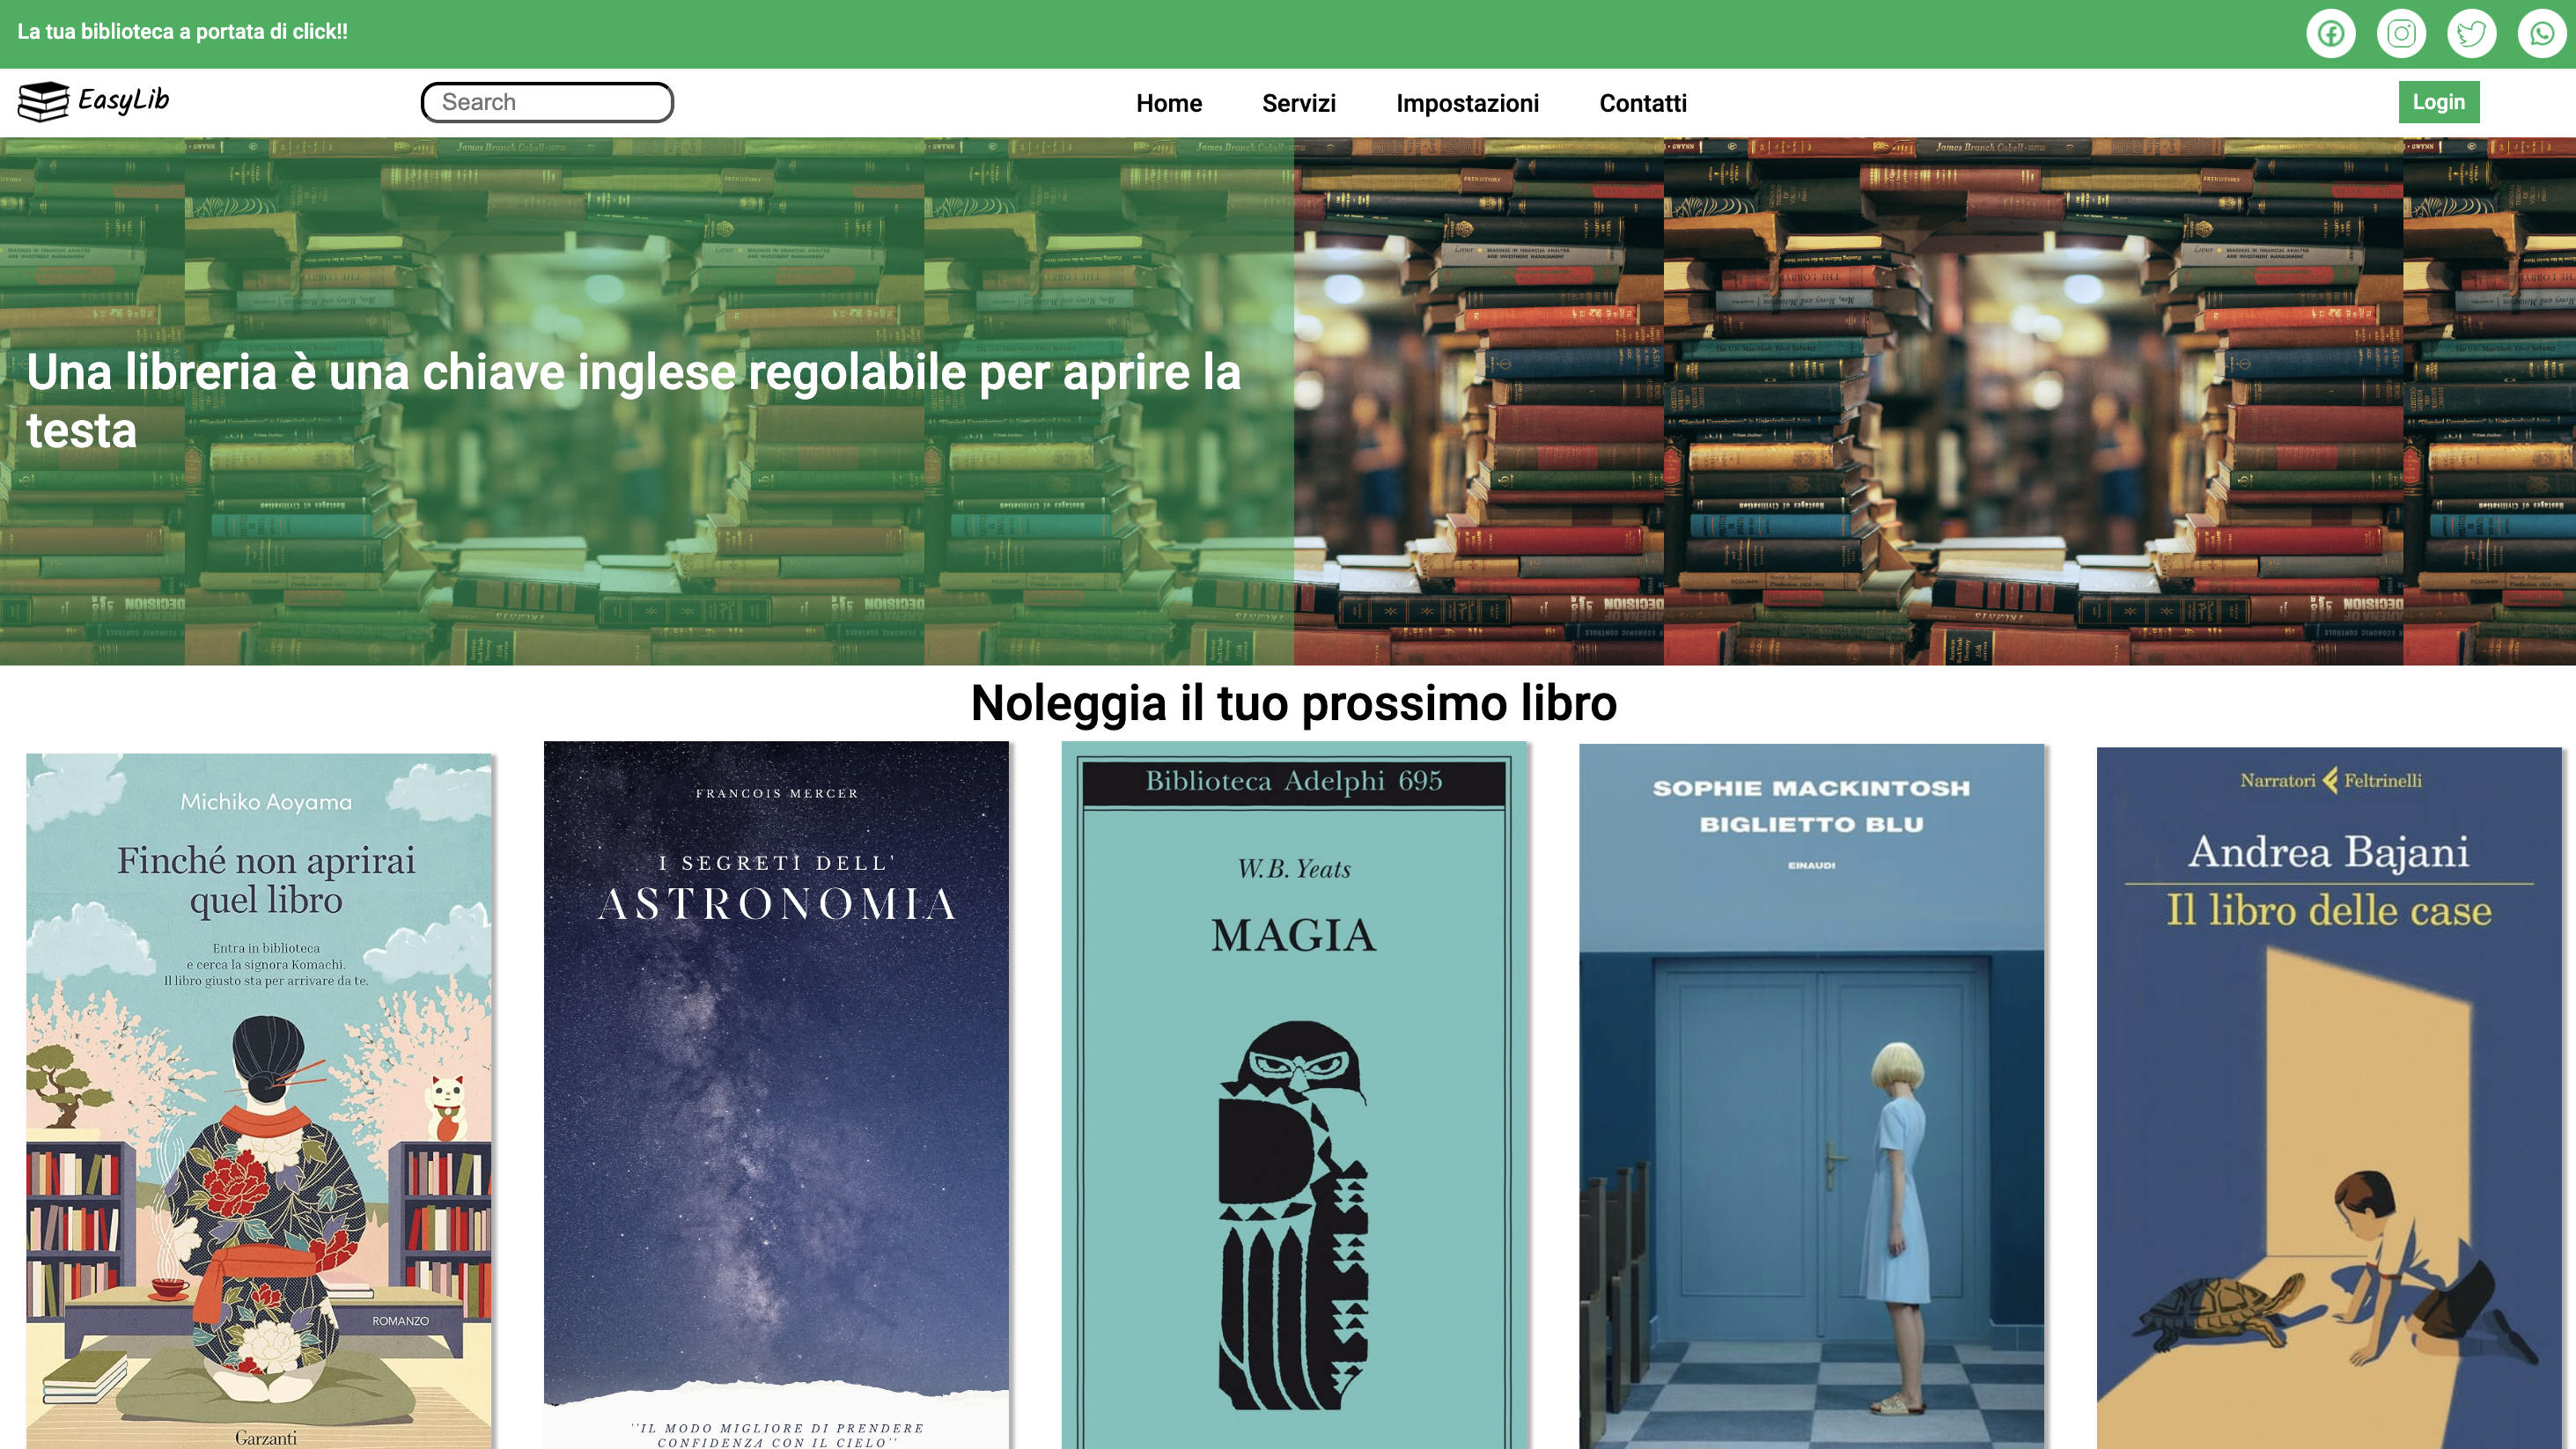
\includegraphics[width=130mm]{D4/Images/Homepage.png}
     \caption{Pagina Homepage}
    \end{figure}

Vediamo subito in alto l'Header contente i link per le varie pagine, ovvero Home, servizi, impostazioni e contatti, oltre al bottone per effettuare il Login.
L'header resterà presente in ogni schermata per facilitare al meglio la navigazione.
 In fondo alla Homepage è presente anche un link diretto all'archivio, come riportato di seguito.
 \begin{figure}[H]
     \centering
     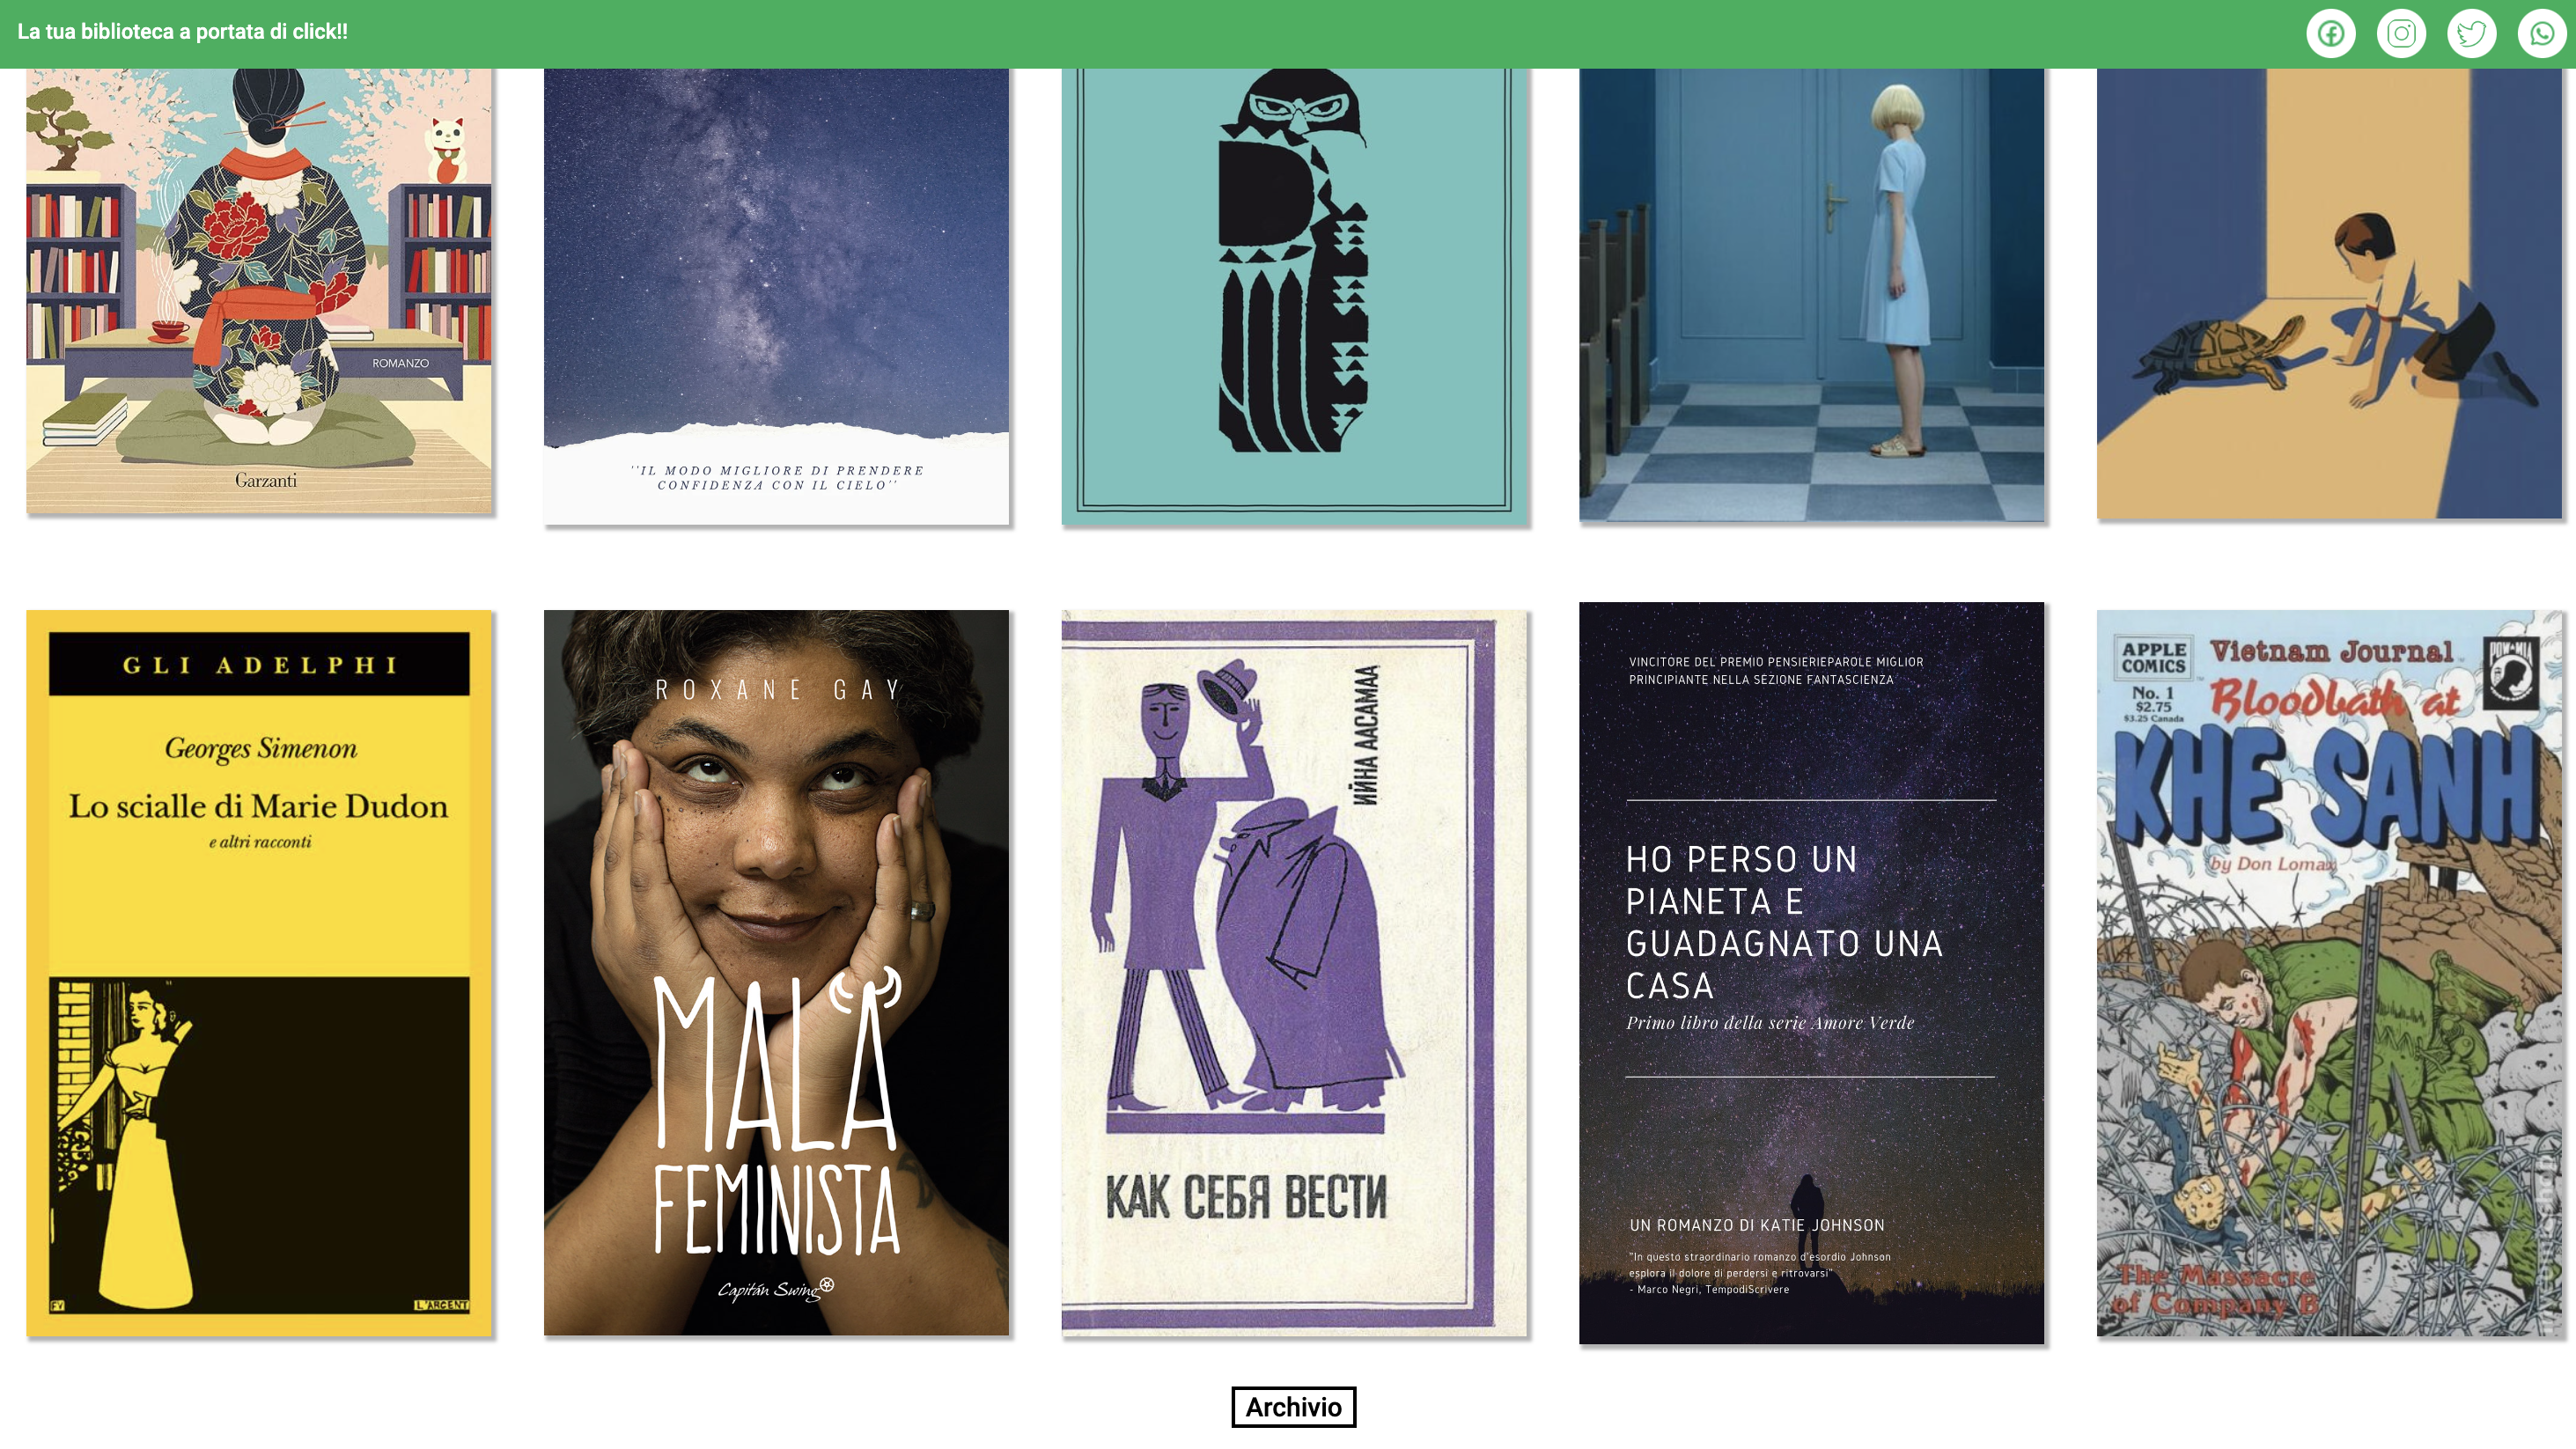
\includegraphics[width=130mm]{D4/Images/Homepage2.png}
     \caption{Pagina Homepage 2}
    \end{figure}

 \subsection{Login}
 La pagina di \textbf{Login} presenta un campo dove inserire la mail e la corrispondente password per gli utenti che si sono già registrati.
    \begin{figure}[H]
     \centering
     \includegraphics[width=130mm]{D4/Images/Login.png}
     \caption{Pagina di Login}
    \end{figure}

\subsection{Registrazione}
La pagina di \textbf{Registrazione} comprende un form da compilare con le varie informazioni per ogni nuovo utente, ovvero: 
\begin{itemize}
    \item Nome
    \item Cognome
    \item Mail
    \item Password
    \item Conferma password
\end{itemize}
La password inoltre deve rispettare i criteri di una password sicura, cioè lunghezza minima 8 caratteri con almeno 1 carattere speciale.
\begin{figure}[H]
    \centering
    \includegraphics[width=130mm]{D4/Images/signUp.png}
    \caption{Pagina di Registrazione}
\end{figure}
\\

\subsection{Archivio} \label{archivio}


La pagina di \textbf{Archivio} presenta tutti i libri presenti all'interno del Database MongoDB con anche la barra di ricerca per cercare uno specifico volume con anche la possibilità di utilizzare dei filtri di ricerca
\begin{figure}[H]
    \centering
    \includegraphics[width=130mm]{D4/Images/Archivio.png}
    \caption{Pagina Archivio} 
\end{figure}
\\

\subsection{Ricerca}
La pagina di ricerca rappresenta i risultati consecutivi a una ricerca fatta utilizzando l'apposita barra oppure selezionando uno dei filtri disponibili nella sidebar, presentando i volumi che corrispondono ai parametri inseriti.
\begin{figure} [H]
    \centering
    \includegraphics[width=130mm]{D4/Images/paginaRicerca.png}
    \caption{Pagina di ricerca}
\end{figure}

\subsection{Servizi}
Nella pagine dei servizi vengono descritti i servizi dell'applicazione nel formato di FAQ.

\begin{figure}[H]
    \centering
    \includegraphics[width=130mm]{D4/Images/Servizi.png}
    \caption{Pagina di Servizi}
\end{figure}

\subsection{Contatti}
La pagina dei \textbf{contatti} presenta un collegamento a Google maps per ottenere le indicazioni per la sede di EasyLIb. In più è presente la mail di riferimento e il numero di telefono della segreteria per avere modalità di  comunicazione con la sede.

\begin{figure}[H]
    \centering
    \includegraphics[width=130mm]{D4/Images/Contatti.png}
    \caption{Pagina dei Contatti}
\end{figure}
\subsection{Impostazioni} La pagina delle impostazioni è suddivisa nelle parti di:
\begin{itemize}
    \item Lingua: dove si può passare dalla lingua italiana a quella inglese.
    \item I miei noleggi: dove si può vedere  i libri noleggiati e terminare la prenotazione.
    \item I miei appuntamenti: dove si possono vedere lo stato degli appuntamenti già riservati.
    \item Pagamenti: dove vengono inviate le multe dal  sistema.
\end{itemize}
 Di seguito alcune immagini della sezione impostazioni.

\begin{figure}[H]
    \centering
    \includegraphics[width=130mm]{D4/Images/Lingua.png}
    \caption{Pagina di impostazioni Lingua}
\end{figure}

\begin{figure}[H]
    \centering
    \includegraphics[width=130mm]{D4/Images/pagamenti.png}
    \caption{Pagina di impostazioni Pagamenti}
\end{figure}

\begin{figure}[H]
    \centering
    \includegraphics[width=130mm]{D4/Images/appuntamenti.png}
    \caption{Pagina di impostazioni appuntamenti}
\end{figure}

\subsection{Appuntamento}
Nella pagina Appuntamento è presente un form da compilare per la prenotazione di un appuntamento in fisico all'interno degli uffici di EasyLib. Le informazioni necessarie per effettuare la prenotazione, e presenti nel form, sono:
\begin{itemize}
    \item Indirizzo email (di un utente già registrato)
    \item Data richiesta dell'appuntamento
    \item L'orario dell'appuntamento
\end{itemize}
in più va specificato fra 2 campi, il motivo della richiesta dell'appuntamento fra quelli presenti, ovvero per restituire un libro  o donarlo.
\begin{figure}[H]
    \centering
    \includegraphics[width=130mm]{D4/Images/Appuntamento.png}
    \caption{Pagina di Prenotazione appuntamenti}
\end{figure}

\subsection{Frontend Admin}
Alla sezione Admin si accede inserendo le apposite credenziali nella fase di login.
Le sue pagine di Frontend presentano alcune differenze con quelle dell'utente normale, le sue pagine di navigazione sono:
\begin{itemize}
    \item Homepage (vedi sezione Homepage \ref{Homepage})
    \item Archivio (vedi sezione Archivio \ref{archivio})
\end{itemize}
Che sono praticamente uguali a quelle disponibili per l'utente normale, e poi:
\begin{itemize}
    \item Donazioni
    \item Utenti
\end{itemize}
Che sono specifiche dell'admin e vengono descritte qui sotto.

\subsubsection{Donazioni Admin}
La pagina di donazioni per l'admin comprende un form necessario all'amministratore per inserire all'interno del sistema i dati del libro donato da un utente.
I campi necessari sono i dati dell'autore, il titolo del volume e il suo genere (si veda figura sottostante).
\begin{figure}[H]
    \centering
    \includegraphics[width=130mm]{D4/Images/Donazioni.png}
    \caption{Pagina di donazioni}
    \label{fig:enter-label}
\end{figure}
La pagina utenti dell'admin, mostra tutti gli utenti registrati e attraverso due bottoni " Apri pagina multe" e "Apri pagina noleggi" si aprono le rispettive pagine che permetto all'admin le sue operazioni di gestione.

\begin{figure}[H]
    \centering
    \includegraphics[width=130mm]{D4/Images/UtentiAdmin.png}
    \caption{Pagina utenti per l'admin}
\end{figure}

\begin{figure}[H]
    \centering
    \includegraphics[width=100mm]{D4/Images/Multa.png}
    \caption{Form per creazione Multa}
\end{figure}

\newpage

\section{Testing}
In questa sezione vengono descritti i casi di test per le  varie API che vengono usate su \textbf{EasyLib}. 
I test sono realizzati utilizzando Jest. 
Di seguito viene descritta la loro realizzazione e il funzionamento.
I casi di test sono divisi in 5 file di tipo test.js a seconda del tipo delle API che vengono testate.
Alla fine della sezione vengono anche mostrati i risultati del test con la copertura del codice diviso per ogni cartella.
\begin{figure}[H]
    \centering
    \includegraphics[width=80mm]{D4/Images/CartellaTest.png}
    \caption{Test Folder}
\end{figure}

Verrà adesso descritta la struttura di un tipico file \textbf{.test.js} per il testing delle API. Tutti i nostri file sono strutturati allo stesso modo, quindi prenderemo come esempio e riporteremo le foto qua sotto, del file \textbf{Utente.test.js}.
\begin{figure}[H]
    \centering
    \includegraphics[width=130mm]{D4/Images/Struttturatest.png}
    \caption{Struttura file test}
    \label{fig:enter-label}
\end{figure}
All'inizio si ha un importazione di \textbf{Mongoose} e del modulo \textbf{Superjest} che effettuano la connessione al database. Viene importato il \textit{jsonwebtoken} che serve per la creazione di un token per alcune API che ne hanno bisogno.

Successivamente ci sono i metodo \textbf{BeforeAll()} che definisce tutto ciò che va fatto nel momento iniziale di esecuzione del file; e \textbf{AfterAll()} che è l'ultimo metodo chiamato che si occupa di chiudere  la connessione al database e disattivare il server.
Questi metodi sono presenti in ogni API

Le API poi vengono testate nelle reciproche parti chiamate dai metodi \textbf{Describe()}

\begin{figure}[H]
    \centering
    \includegraphics[width=130mm]{D4/Images/CasiTest.png}
    \caption{Casi di test Utente}
\end{figure}

Di seguito viene anche riportato un esempio di un metodo describe(),
in questo caso per semplicità viene riportato il test di \textbf{/deleteAppuntamento}

\begin{figure}[H]
    \centering
    \includegraphics[width=100mm]{D4/Images/describetest.png}
    \caption{Testing /deleteAppuntamento}
\end{figure}

In questa API i casi di test sono 2: uno di successo in cui viene passata una mail con un appuntamento fissato che andrà poi cancellato, con response code \textbf{200}.
E uno in caso di insuccesso dove alla mail passata come input non corrisponde nessun appuntamento, il response code  \textbf{404}.
\subsection{Risultati del test}
Per fare il testing abbiamo aggiunto il seguente script al file package.json : 'test':'jest --coverage --detectOpenHandles'.
Tramite il comando npm test, fatto partire dalla root del progetto otterremo tutti i risultati dei test definiti nei file '.test.js'.

La flag --coverage di jest serve a creare dei report finali del nostro testing, mentre la flag --detectOpenHandles serve a identificare elementi che non permettono al testing di terminare.
I risultati:

\begin{figure}[H]
    \centering
    \includegraphics[width=80mm]{D4/Images/TestSuites.png}
    \caption{Test Suites}
\end{figure}

Le 5 suites definite e i 53 test case, definiti nelle funzioni test(), sono stati eseguiti e risultano passati.

Il report dei risultati del testing generato da coverage si può trovare nel file \textbf{index.html}, locato, a partire della root del progetto, nella cartella \textbf{coverage/lvcon-report/}. La pagina ipertestuale risultante è la seguente:

\begin{figure}[H]
    \centering
    \includegraphics[width=130mm]{D4/Images/CoverageAllFiles.png}
    \caption{Coverage Progetto}
\end{figure}

Questa prima pagina presenta un riassunto della copertura di tutte le funzioni, i branches, gli statements e le linee di codice del progetto prese in carico dal testing.

La cartella che ci interessa è Backend/controllers, che è quella dove abbiamo definito tutte le api.
Si nota che abbiamo circa un 93\% di copertura per i branches, le linee di codice e gli statements, mentre le funzioni sono coperte al 100\%.

Cliccando sopra Backend/controllers ci viene mostrata la pagina seguente,  che rappresenta il coverage delle api:

\begin{figure}[H]
    \centering
    \includegraphics[width=130mm]{D4/Images/CoverageControllers.png}
    \caption{Coverage delle API}
\end{figure}

Si nota che c'è un'oscillazione tra le percentuali della copertura, questa differenza tra questi numeri è data da errori del seguente tipo, che non sono dipendenti da noi, ma dal server:

\begin{figure}[H]
    \centering
    \includegraphics[width=130mm]{D4/Images/CoverageError500.png}
    \caption{Errori del server}
\end{figure}

Inoltre nelle API di creazione di un nuovo libro e nuovo utente abbiamo utilizzato una funzione specializzata per l'id dei rispettivi, i.e. la mancata copertura delle seguenti linee di codice:

\begin{figure}[H]
    \centering
    \includegraphics[width=130mm]{D4/Images/CoverageID.png}
    \caption{Copertura di ID utente e libro non presente}
\end{figure}


Altro problema riscontrato è nelle API di getAll dei libri e degli utenti:

\begin{figure}[H]
    \centering
    \includegraphics[width=130mm]{D4/Images/ErroreCovGetAll.png}
    \caption{Esempio dell'API su utente}
\end{figure}

per far si che queste linee vengano coperte bisognerebbe avere il database vuoto o inesistente, e nel nostro caso non lo è mai stato.
Per l'API getAllBooks è la stessa cosa.


Abbiamo anche usato delle funzioni ausiliare per la validazione della mail e della password, definite in 'Backend/auxiliaries/', qui sotto il coverage:

\begin{figure}[H]
    \centering
    \includegraphics[width=130mm]{D4/Images/CoverageAuxiliaries.png}
    \caption{Coverage Progetto}
\end{figure}

\newpage

\section{GitHub repository and Deployment}
Al seguente URL è presente la repository Github del nostro progetto:
\begin{center}
\url{https://github.com/orgs/G06-Progetto-IS/repositories}.\\
\end{center}

Il nome della cartella è \textbf{G06-Progetto-IS}. Nella sezione \textbf{Deliverables} sono presenti i vari deliverables da consegnare.
Nella repository \textbf{Documentazione} sono presenti le bozze dei documenti iniziali, in seguito abbiamo iniziato ad utilizzare il sito \textbf{Overleaf} per produrre documenti .pdf usando il linguaggio \LaTeX. Inoltre sono presenti i vari aggiornamenti delle ore di lavoro.
Nella repository \textbf{Backend} è presente tutto il codice relativo alla nostra applicazione, FrontEnd compreso.
Mentre nella repository \textbf{Frontend} è presente solo il codice HTML e CSS.

\subsection{Deployment}
Il deployment è stato effettuato utilizzando \url{https://render.com} e la nostra applicazione è raggiungibile utilizzando l' URL: 
\begin{center}
 \url{https://easylib-wf03.onrender.com}  
\end{center}

\noindent \textbf{Nota}: Il primo caricamento del nostro sito a causa dell'utilizzo del servizio 'free' di 'Render' può richiedere fino a 50 secondi. Una volta eseguito il primo caricamento poi girerà tranquillamente con dei tempi di attesa minori di 1 secondo.\\

La documentazione delle API svolta con Swagger è raggiungibile tramite l'URL: 
\begin{center}
  \url{https://easylib-wf03.onrender.com/api-docs}  
\end{center}
\textbf{Selezionare lo schema HTTPS per chiamare le varie API.}

\subsubsection{Eseguire in locale}
Nel caso in cui si voglia eseguire il server sulla propria macchina, bisgna prima di tutto usare l'URL: \url{https://github.com/G06-Progetto-IS/Backend} e clonare la repository sulla propria macchina.
Successivamente aprire la cartella Backend utilizzando \textbf{Visual studio Code}, eseguire su terminale il comando \textbf{npm start}.
Non appena vengono stampate in console le seguenti righe:
Server in ascolto sulla porta: 3000
MongoDB Connection -- Ready state is: 1
è possibile collegarsi tramite il browser alla webApp, utilizzando l'URL \url{http://localhost:3000/} si riuscirà a navigare sul sito.

\textbf{Note per la documentazione}
La documentazione delle API svolta con Swagger è raggiungibile tramite l'URL: 
\begin{center}
  \url{http://localhost:3000/api-docs}  
\end{center}
\textbf{Selezionare lo schema HTTP per chiamare le varie API.}.

\end{document}